\chapter{OFDM Basics and Impairments}\label{sec:basic}

In this chapter the basic principles of \gls{ofdm} baseband signal processing are given and an appropriate discrete-time OFDM system model is introduced. In the following section impact and prevention of synchronization errors and equalization are explained. Finally, digital modulations commonly used in wireless transmission standards are described in~\cref{sec:cohmod}.

\begin{figure}[htbp]
\centering
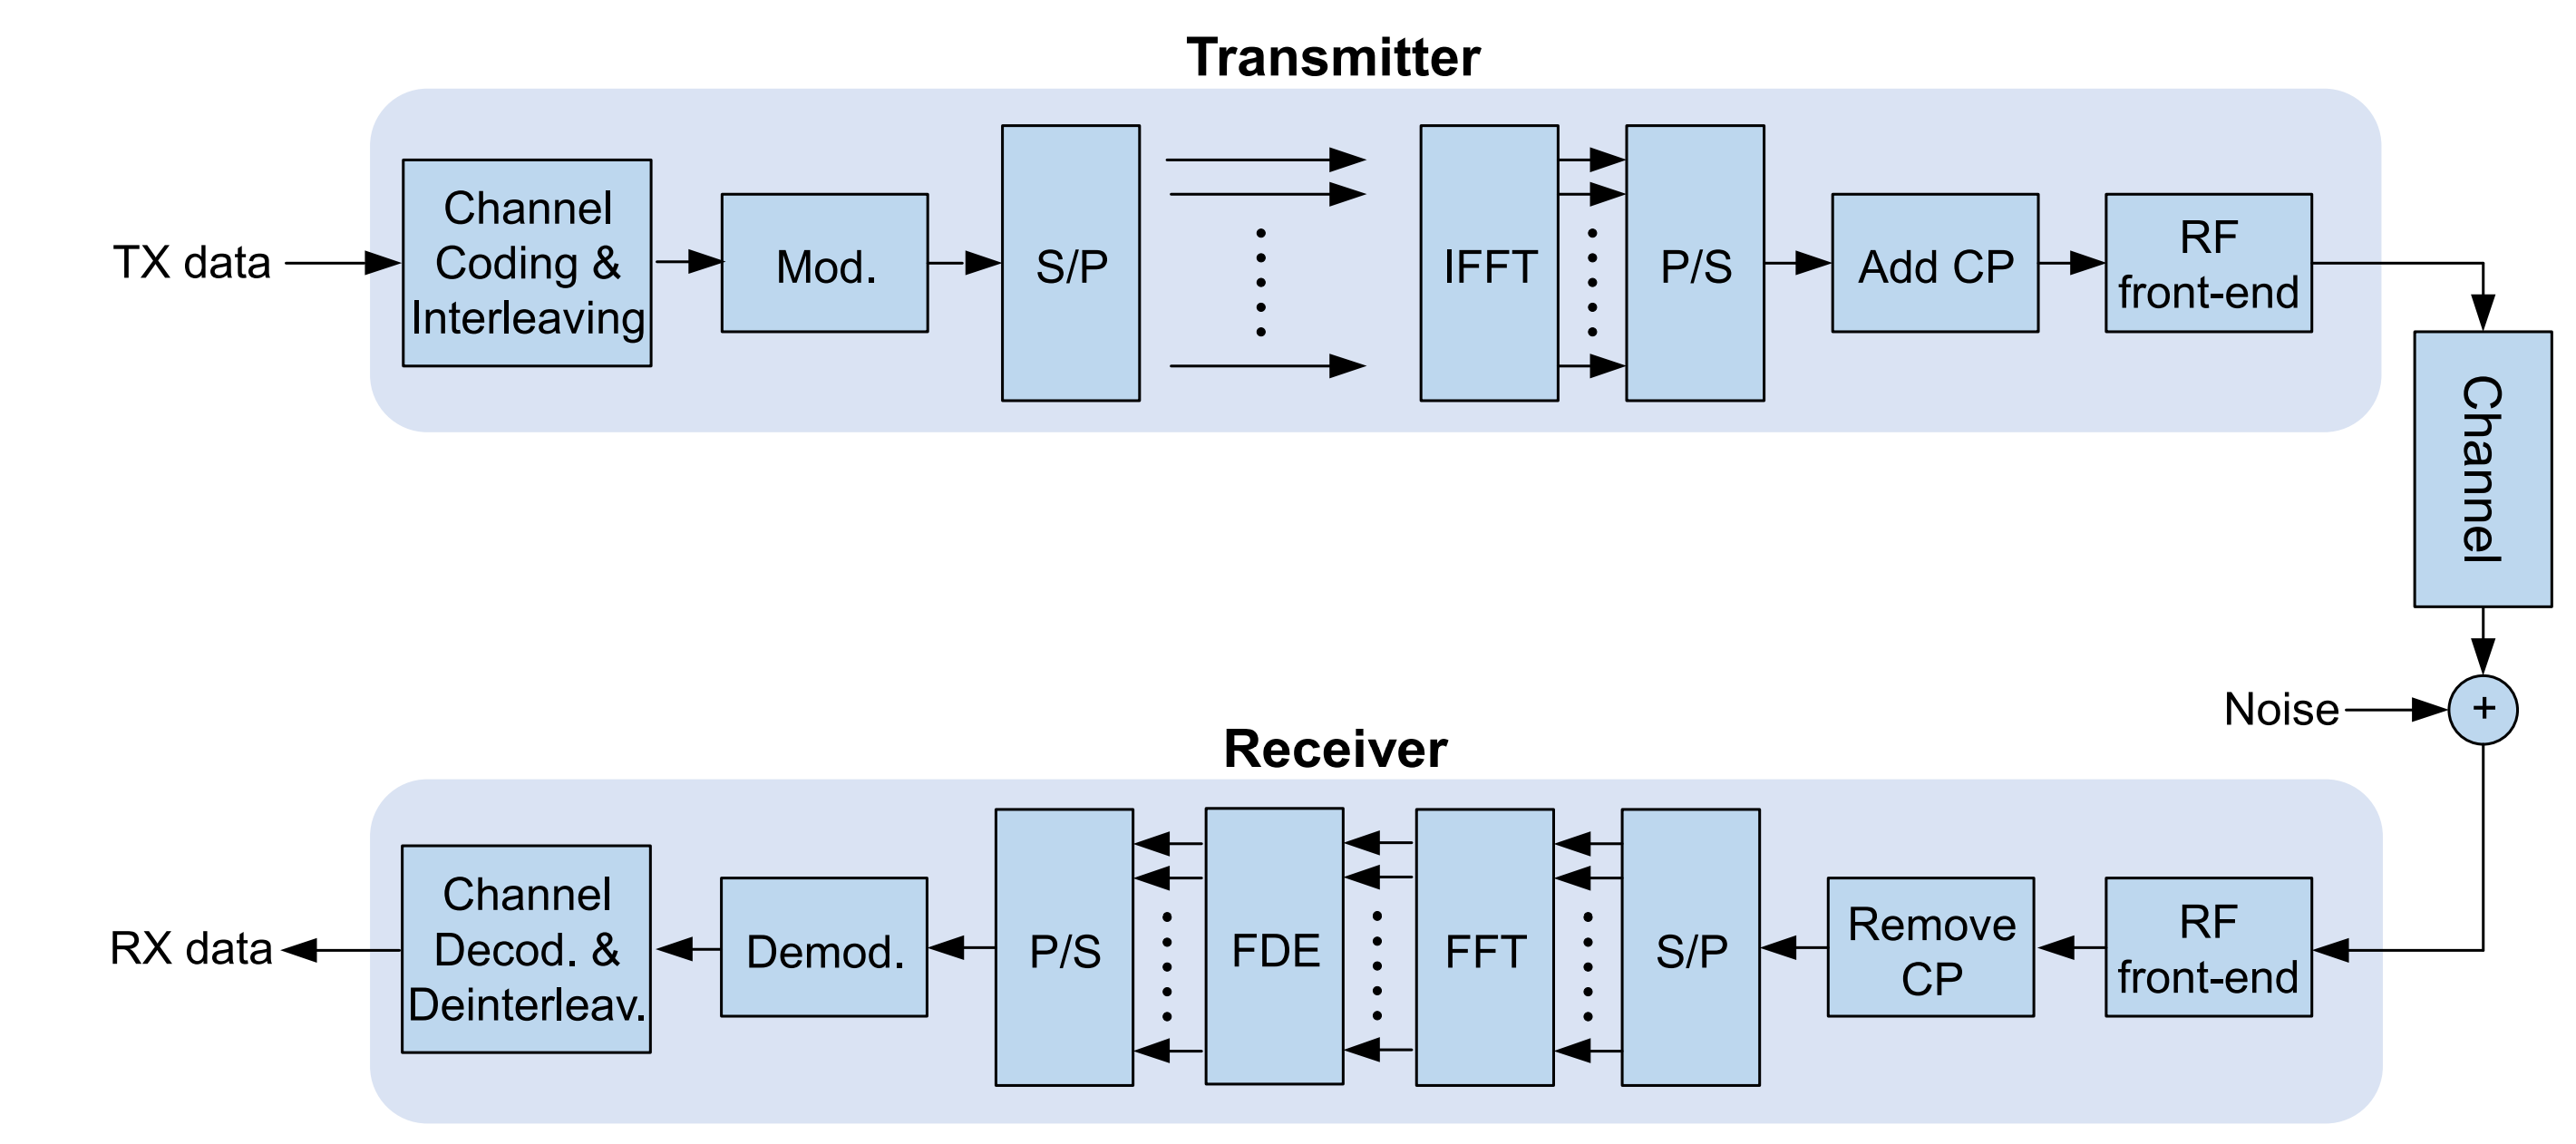
\includegraphics[width=\linewidth]{figs/ofdm_block.png}
\caption{Block diagram of a typical \gls{ofdm} system (image from~\cite{arslan2020flexible})}\label{fig:block_diagram}
\end{figure}

\section{The basics (in laymen terms)}\label{sec:ofdm-laymen}
Imagine you have a fast internet connection, and you want to send a large file to a friend. Instead of sending the entire file in one go, you decide to break it into smaller chunks and send them separately. This makes it easier to manage and lessens the chance of losing all the data if something goes wrong during transmission. This is the main operating principle of \gls{ofdm}.

\subsection{Key features}

\begin{itemize}
    \item[]\textbf{Frequency Division Multiplexing}\\ \Gls{ofdm} combines the principles of multiplexing and modulation. Multiplexing is the technique of combining multiple signals into one signal for transmission, while modulation involves modifying the properties of a carrier signal to encode information. In \gls{ofdm}, each subchannel is modulated independently using a technique like \gls{qam} (see \cref{sec:cohmod}), and then all the modulated subchannels are combined for transmission.
    \item[]\textbf{Orthogonality}\\
In \gls{fdm}, the subchannels are typically close to each other in frequency, which can lead to interference. \gls{ofdm} employs a clever technique called orthogonalization\footnote{In mathematics, two functions are orthogonal if their inner product (the integral of their product over a given interval) is zero.}, where the subchannels are spaced apart at precise intervals, ensuring that they don't interfere with each other. It's akin to having lanes on a highway spaced far enough apart that cars in one lane don't disrupt those in adjacent lanes.
\item[]\textbf{Multiplexing}\\
After orthogonalization, multiple streams of data can be transmitted simultaneously over the different subchannels. Each subchannel acts as a separate communication path, allowing for efficient use of the available spectrum. If the subchannels are used by multiple users, this technique is called \gls{ofdma}.
\end{itemize}

\subsection{Benefits of OFDM}

\begin{itemize}
    \item[] \textbf{Spectral Efficiency}\\
    By dividing the available bandwidth into smaller subchannels, \gls{ofdm} allows for efficient use of the spectrum. This enables higher data rates compared to traditional single-carrier modulation techniques.
    \item[] \textbf{Robustness}\\
    \Gls{ofdm} is inherently robust against frequency-selective fading~\cite{MCMorelli}, which occurs when different frequencies in the signal experience different levels of attenuation or delay. Since \gls{ofdm} divides the signal into multiple subchannels, even if some subchannels are affected by fading, others may still carry useful data.
    \item[] \textbf{Flexibility}\\
    \Gls{ofdm} can adapt to changing channel conditions by adjusting parameters such as subchannel spacing and modulation scheme. This flexibility makes it suitable for a wide range of communication systems.
\end{itemize}


\section{The OFDM System}\label{sec:ofdm-overview}

The block diagram of a typical \gls{ofdm} system is shown in~\cref{fig:block_diagram}. The main idea behind \gls{ofdm} is to divide a high-rate encoded data stream (with symbol time $T_S$) into $N$ parallel substreams (with symbol time $T = NT_S$) that are modulated onto $N$ orthogonal carriers (referred to as subcarriers). This operation is easily implemented in the discrete time domain through an $N$-point \gls{idft} unit and the result is transmitted serially. At the receiver, the information is recovered by performing a \gls{dft} on the received block of signal samples.
%

%
%
The data transmission in \gls{ofdm} systems is accomplished in a symbolwise fashion, where each OFDM symbol conveys~$N$ (possibly coded) complex data symbols. 

\subsection{The Wireless Channel -- A short summary}
In wireless communication systems, transmitted signals are typically reflected, diffracted, and scattered, arriving at the receiver along multiple paths with different delays, amplitudes, and phases as illustrated in~\cref{fig:multipath}. This leads to an overlapping of different copies of the same signal on the receiver side differing in their amplitude, time of arrival and phase. 
%
\begin{figure}[htbp]
\centering
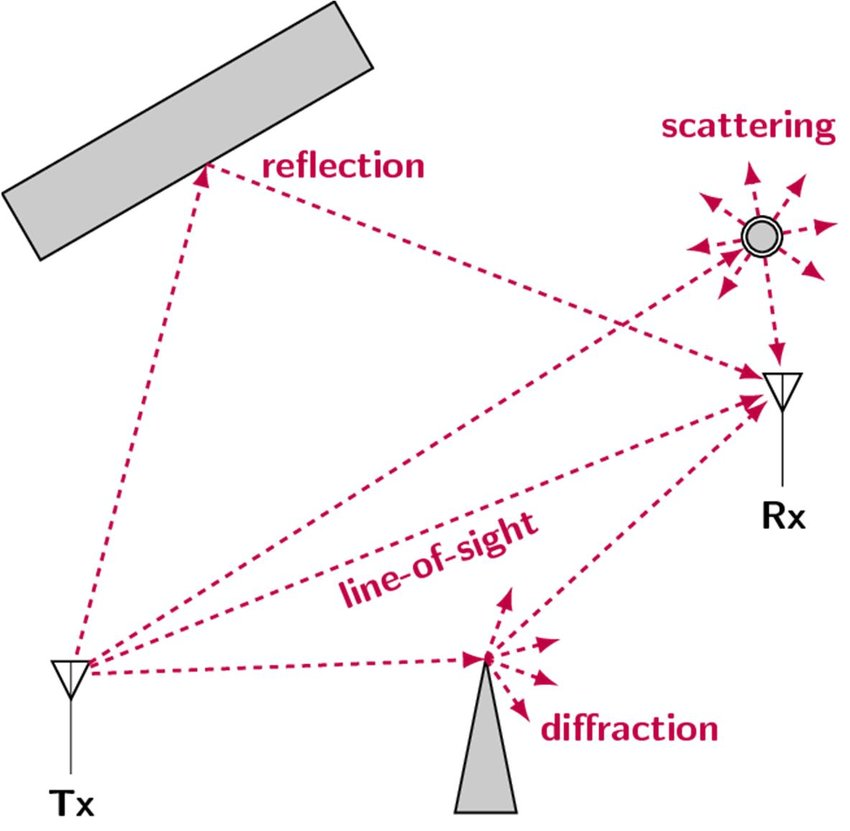
\includegraphics[width=0.4\textwidth]{figs/Some-effects-causing-multipath-propagation.png}
\caption{The basic principle of multipath propagation (image form~\cite{milosevic2021key})}\label{fig:multipath}
\end{figure}
%
A common model to describe the wireless channel makes use of the \textit{channel impulse response} (time domain), written as,
\begin{equation}
h(l)=\alpha(l) e^{j\theta(l)},
\end{equation} for $l = 0,\ldots,L-1 $, where $L$ presents the total number of received signal paths, while $\alpha(l)$ and $ \theta(l)$ are attenuation and phase shift of the $l$th path, respectively. The differences in the time of arrival are eliminated by the cyclic prefix, which is described in the next section. One of the effects of the reception of multiple overlapping copies, i.e., multipath, is frequency selective fading. From the signal's perspective, the signal experiences different attenuation for different frequencies, complicating mitigation of these unwanted effects. This is the reason why \gls{ofdm} is used, as it ''splits'' the spectrum in several subchannels, allowing to use single-tap equalizers to resolve frequency-selective fading. See~\cref{ss:equ} for more details.


As a consequence of the time dispersion associated with the frequency-selective channel, contiguous \gls{ofdm} symbols may partially overlap in time-domain. This phenomenon results into \gls{isi}, with ensuing limitations of the system performance. The common approach to mitigate \gls{isi} is to introduce a guard interval of appropriate length between adjacent symbols. In practice, the guard interval is obtained by duplicating the last part of the \gls{ofdm} symbol and, for this reason, is commonly referred to as \gls{cp}.
As illustrated in~\cref{fig:cp}, the \gls{cp} is appended in front of the corresponding \gls{idft} output. This results into an extended \gls{ofdm} symbol consisted of the \gls{cp} and original \gls{ofdm} symbol. The \gls{isi} can be removed as long as the \gls{cp} length is properly designed according to the channel delay spread.

Referring to~\cref{fig:block_diagram}, lets concentrate on the receiver. The first operation is the \gls{cp} removal, which is simply accomplished by discarding the first $N_G$ samples of the considered segment (the lenght of the \gls{cp}). The remaining $N$ samples are fed to a \gls{dft} and the corresponding output is subsequently passed to the \gls{fde}. Assuming that synchronization has already been established and the \gls{cp} is sufficiently long to eliminate the \gls{isi}, only a one-tap complex-valued multiplier is required to compensate for the channel distortion over each subcarrier, which will be further described in~\cref{ss:equ}. To better understand this fundamental property of \gls{ofdm}, however, we need to introduce the mathematical model of the communication scheme depicted in ~\cref{fig:block_diagram}.
%
\begin{figure}[thb]
\centering
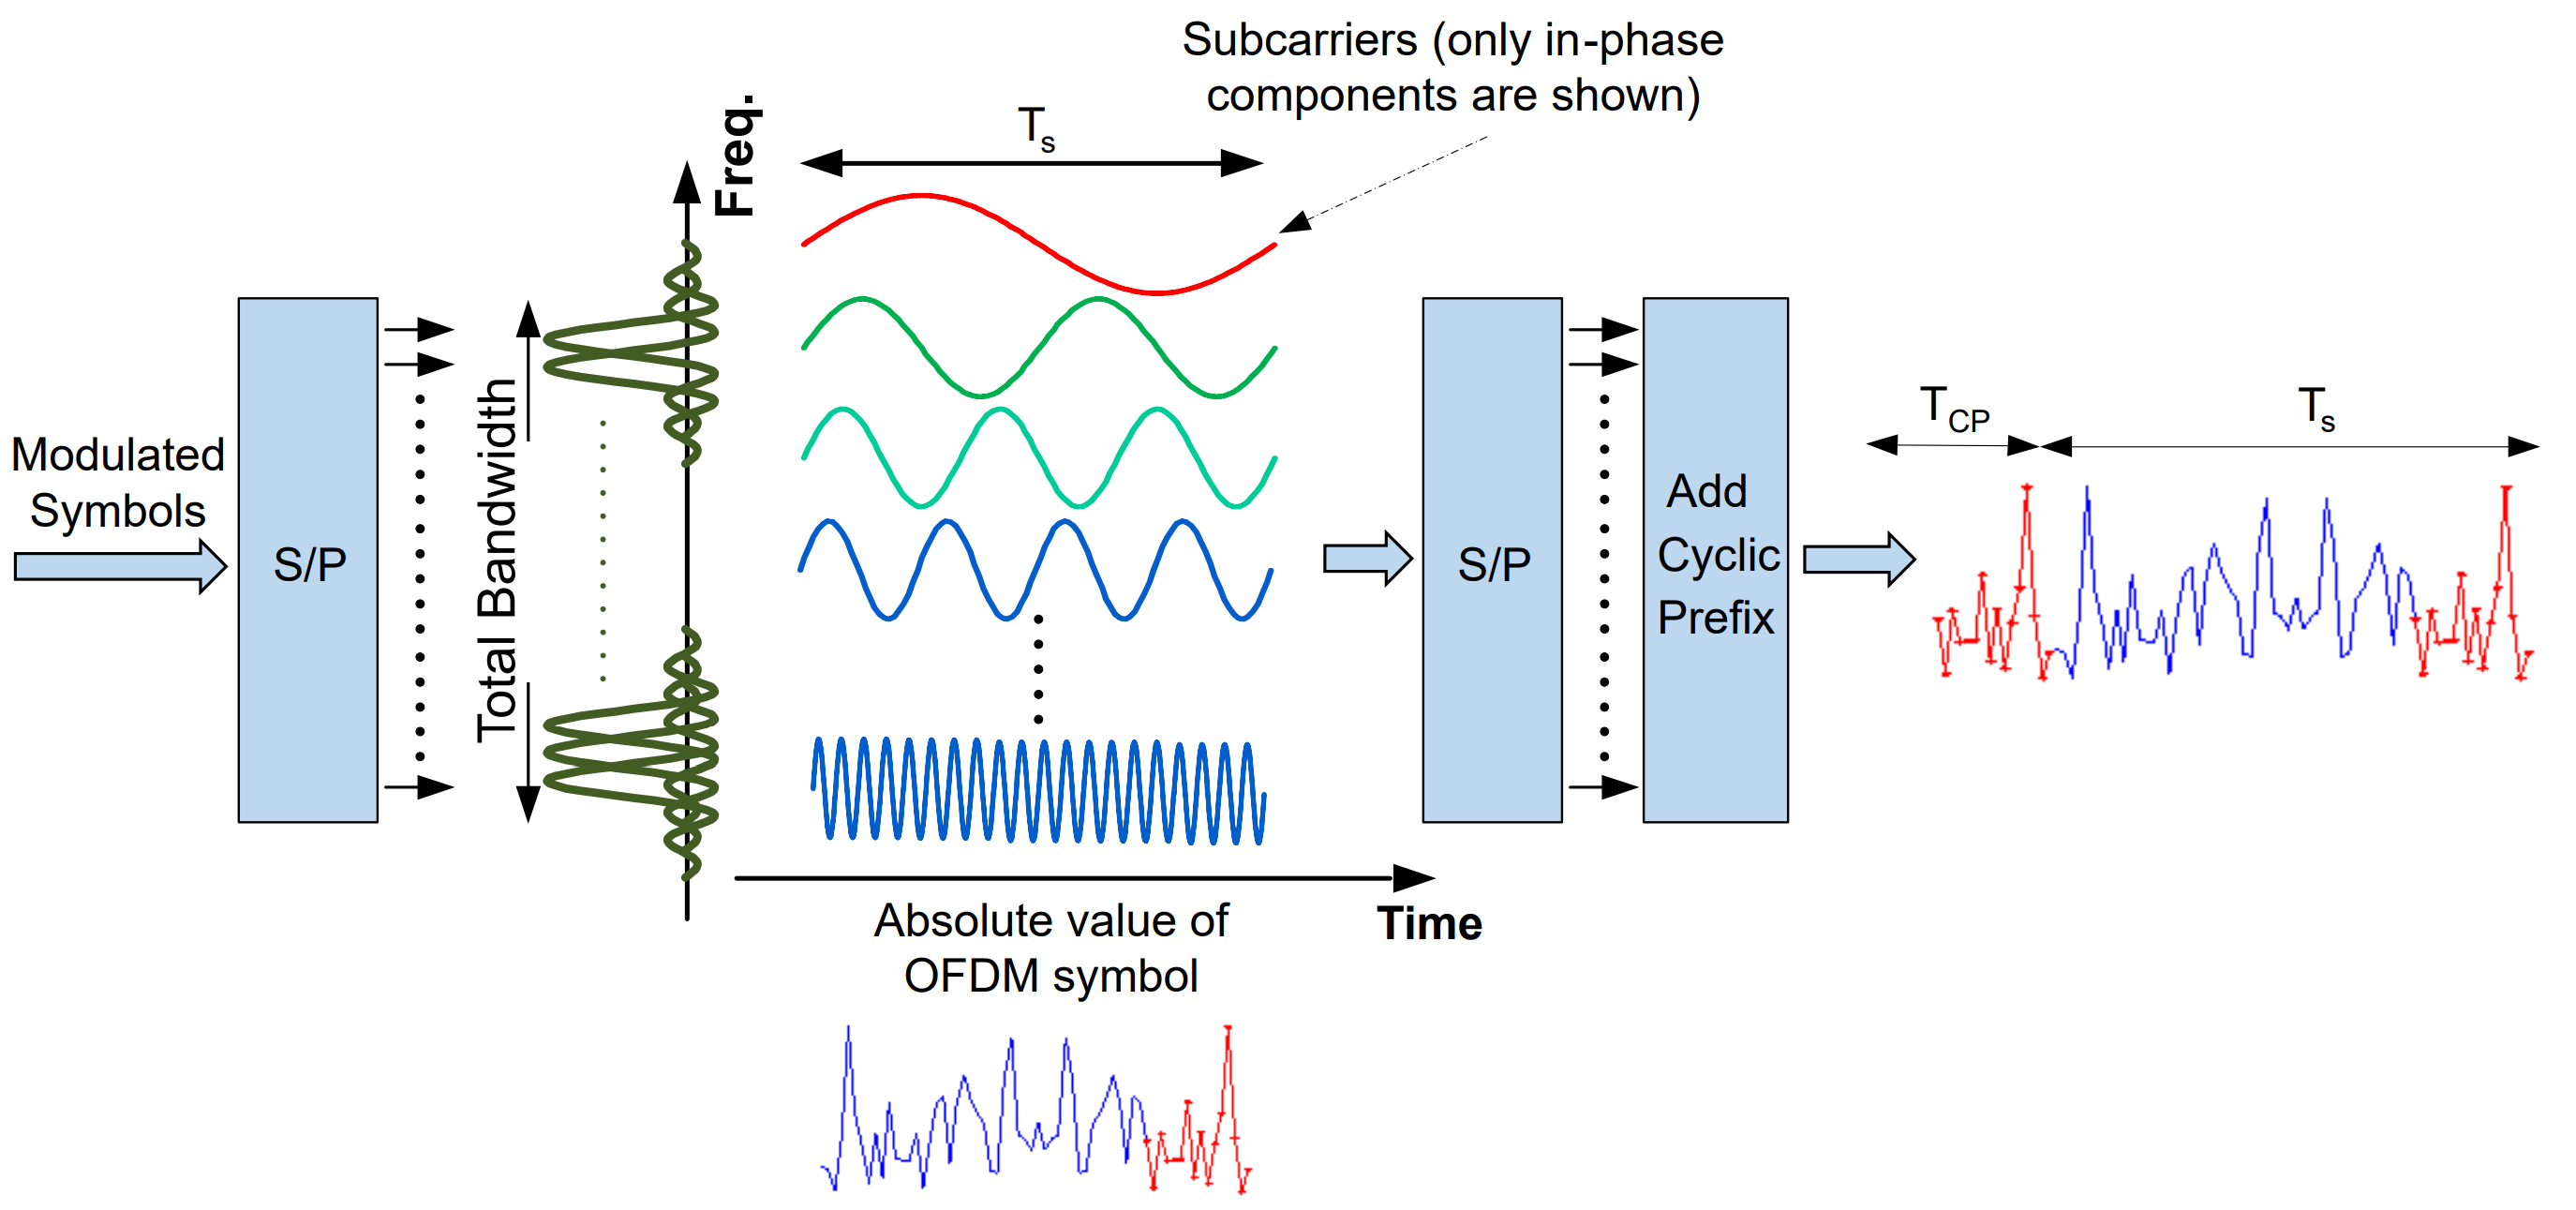
\includegraphics[width=1.00\linewidth]{figs/cp-ofdm_block.png}
\caption{Structure of an OFDM symbol (image from~\cite{arslan2020flexible})}\label{fig:cp}
\end{figure}



\section{Discrete-time OFDM System Model}\label{sec:discmod}

Since \gls{ofdm} is a block based communication model, a serial data stream is converted into parallel blocks of size N and \gls{idft} is applied to obtain time-domain \gls{ofdm} symbols. 
% Let denote $\mathbf{C_i}=\left[ C_i(0),C_i(1),\dots,C_i(N-1)\right]^T$ the $i$th block of data at the IDFT input, with length $N$ where $(.)^T$ represents the transponse operator. 
Complex data symbols $C_i(n)$, for $n=0,\ldots,N-1$, within the $i$th OFDM symbol are taken from either a \gls{psk} or \gls{qam} constellation. Then, time domain representation of the $i$th OFDM symbol after \gls{idft} and \gls{cp} insertion is given by
%
\begin{equation}\label{IDFT}
c_i(k)= 
\begin{cases}
   \sum_{n=0}^{N-1}{C_i(n)e^{j2\pi kn/N}},& -N_G \leq k \leq N-1\\
   0,&\text{else}
\end{cases},
\end{equation}
%
where $N_G$ is the length of the \gls{cp} which is an important design parameter of the \gls{ofdm} system that defines the maximum acceptable length of channel impulse response. Furthermore, the transmitted signal can be obtained by concatenating \gls{ofdm} symbols in time domain as

\begin{equation}\label{concat}
c(k)=\sum_i{c_i(k -iN_T)}.
\end{equation} 

In addition to multipath effects, additive noise is introduced to the transmitted signal. The main sources of additive noise are thermal background noise, electrical noise in the receiver amplifiers, and interference \cite{StuberOFDM}. The noise decreases the \gls{snr} of the received signal, resulting in a decreased performance. The total effective noise at the receiver of an \gls{ofdm} system can be modeled as \gls{awgn} with a uniform spectral density and zero-mean Gaussian probability distribution. The time domain noise samples are represented by $w(k) \sim CN(0,\sigma_w^2)$, where $\sigma_w^2$ denotes the noise variance and $0$ the mean of the circular symmetric complex distribution. Therefore, the discrete-time model of received \gls{ofdm} signals can be written as,
\begin{equation}
\label{eqn:multipath}
y(k) = \sum_{l = 0}^{L-1} h(l)c(k-l) + w(k).
\end{equation}
%
Multipath propagation and additive noise affect the signal significantly, corrupting the signal and often placing limitations on the performance of the system.








\section{OFDM System Impairments}\label{sec:sysimp}
Since timing and frequency errors in multi-carrier systems destroy orthogonality among subcarriers which results in large performance degradations, synchronization of time and frequency plays a major role in the design of a digital communication system. Essentially, this function aims at retrieving some reference parameters from the received signal that are necessary for reliable data detection. In an \gls{ofdm} system, the following synchronization tasks can be identified \cite{MCMorelli}:
\begin{itemize}
 \item \textit{sampling clock synchronization}: in practical systems the sampling clock frequency at the receiver is slightly different from the corresponding frequency at the transmitter. This produces \gls{ici} at the output of the receiver's \gls{dft} with a corresponding degradation of the system performance. The purpose of a sampling clock synchronization is to limit this impairment to a tolerable level.
\item \textit{timing synchronization}: the goal of this operation is to identify the starting point of each received OFDM symbol in order to find the correct position of the \gls{dft} window. In burst-mode transmissions timing synchronization is also used to locate the start of the frame (frame synchronization) which is a collection of OFDM symbols.
\item \textit{frequency synchronization}: a frequency error between the local oscillators at the transmitter and receiver results in a loss of orthogonality among subcarriers with ensuing limitations of the system performance. Frequency synchronization aims at restoring orthogonality by compensating for any frequency offset caused by oscillator inaccuracies.
% or Doppler shifts.
\end{itemize}

The block diagram of the receiver is depicted in~\cref{fig:receiver}. In the analog frontend, the incoming waveform $r_{RF}(t)$ is filtered and down-converted to baseband using two quadrature sinusoids generated by a \gls{lo}. The baseband signal is then passed to the \gls{adc}, where it is sampled with frequency $f_s = 1/T_s$. Due to Doppler shifts and/or oscillator instabilities, the frequency $f_{LO}$ of the \gls{lo} is not exactly equal to the received carrier frequency $f_c$. The difference $f_d = f_c - f_{LO}$ is referred to as \gls{cfo}, or shorter frequency offset, causing a phase shift of $2\pi kf_d$\footnote{Notice that this phase shift is not time dependent (if $f_d$ is constant) and is different for each subcarrier $k$.}. Therefore, the received baseband signal can be expressed as
%
\begin{equation}
\label{eqn:received_time_freqshift}
r(k) =y(k)e^{j2\pi \varepsilon k/N} 
\end{equation}
%
where

\begin{equation}
\label{eqn:norm_freq_off}
\varepsilon = Nf_dT_s
\end{equation}

is the frequency offset normalized to subcarrier spacing $\Delta f =1/(NT_s)$.
In addition, since the time scales at the transmitter and the receiver are not perfectly aligned, at the start-up the receiver does not know where the OFDM symbols start and, accordingly, the \gls{dft} window will be placed in a wrong position. As it will be shown later, since small (fractional) timing errors do not produce any degradation of the system performance, it suffices to estimate the beginning of each received OFDM symbol within one sampling period.
%
\begin{figure}[thb]
\centering
\includegraphics[width=1.00\linewidth]{syncstages.eps}
\caption{Block diagram of a basic OFDM receiver\label{fig:receiver} }
\end{figure}
%
Let $\Delta k$ denotes the number of samples by which the receive time scale is shifted from its ideal setting. The samples from ADC are thus expressed by
%
\begin{equation}
\label{eqn:received_time_frtime}
r(k) =e^{j2\pi \varepsilon k/N}y(k-\Delta k) + w(k).
\end{equation}
%
Replacing (\ref{concat}) and (\ref{eqn:multipath}) in (\ref{eqn:received_time_frtime}), samples are given as
%
\begin{equation}
\label{eqn:received_time_all}
r(k) =e^{j2\pi \varepsilon k/N} \sum_i{}\sum_{l=0}^{L-1}{h(l)c_i(k-l-\Delta k-iN_T)}+ w(k).
\end{equation}

The frequency and timing synchronization units shown in ~\cref{fig:receiver} employ the received samples $r(k)$ to compute estimates of $\varepsilon$ and $\Delta k$, noted as $\hat{\varepsilon}$ and $\hat{\Delta k}$. The former is used to counter-rotate $r(k) $ at an angular speed $2\pi \hat{\varepsilon} k/N$ (frequency correction) using \gls{cfo}, while the timing estimate is exploited to achieve the correct position of the received signal within the \gls{dft} window (timing correction). Specifically, the samples $r(k)$ with indices $iN_T + \Delta k \leq k \leq iN_T + \Delta k + N - 1$ are fed to the \gls{dft} device and the corresponding output is used to detect the data symbols conveyed by the $i$th OFDM block.
%The DFT output can also be exploited to track and compensate for small short-term variations of the frequency error (fine-frequency estimation).
\subsection{Effects of Frequency Offset}

In order to assess the impact of a frequency error on the system performance, we assume ideal timing synchronization and let $\Delta k = 0$ and $N_g \geq L-1$.
At the receiver, the \gls{dft} output for the $i$th OFDM symbol is computed as
%
\begin{equation}
\label{eqn:received_freq_freqoff}
R_i(n) =\frac{1}{N} \sum_{k=0}^{N-1} r(k+iN_T)e^{-j2\pi k n/N} ,\ 0 \leq n \leq N-1
\end{equation}
%
Substituting (\ref{eqn:received_time_all}) into (\ref{eqn:received_freq_freqoff}) we get
%
\begin{equation}
\label{eqn:received_freq_devel}
\begin{split}
R_i(n)
&=\frac{1}{N}\sum_{k=0}^{N-1}{\left[ e^{j2\pi \varepsilon(k+iN_T)/N}\sum_{l=0}^{L-1} {h(l)c_i(k-l)}+w(k)\right] e^{-j2\pi kn/N}}\\
&=\frac{1}{N}e^{j\varphi_i}\sum_{k=0}^{N-1}{e^{j2\pi k(\varepsilon-n)/N}}\sum_{l=0}^{L-1} {h(l)\sum_{m=0}^{N-1}{C_i(m)e^{j2\pi (k-l)m/N}}}+W_i(n)\\
&=\frac{1}{N}e^{j\varphi_i} \sum_{m=0}^{N-1} \left\lbrace \sum_{l=0}^{L-1} h(l)e^{j2\pi lm/N}\right\rbrace C_i(m)\sum_{k=0}^{N-1} e^{-j2\pi k (m+\varepsilon -n)/N}+W_i(n)\\
&=\frac{1}{N}e^{j\varphi_i} \sum_{m=0}^{N-1} H(m) C_i(m)\sum_{k=0}^{N-1} e^{j2\pi k (m+\varepsilon -n)/N} +W_i(n)
\end{split}
\end{equation}
%
%
where $\varphi_i = 2\pi i \varepsilon N_T/N$, $W_i(n)$ is Gaussian distributed thermal noise with variance $\sigma_{w}^2$ derived as
%
\begin{equation}
\label{eqn:noise_freq}
W_i(n) =\frac{1}{N} \sum_{k=0}^{N-1} w(k)e^{-j2\pi k n/N} ,\ 0 \leq n \leq N-1
\end{equation}
%
and $H(m)$ is {channel frequency response}\index{Channel frequency response} defined as DFT of channel impulse response given as
%
\begin{equation}
\label{eqn:CFR}
H(m) =\sum_{l=0}^{L-1} h(l)e^{-j2\pi l m/N} ,\ 0 \leq m \leq N-1.
\end{equation}
%
Performing standard mathematical manipulations (\ref{eqn:received_freq_devel}) is derived to
%
\begin{equation}
\label{eqn:received_freq_developed}
R_i(n)=e^{j\varphi_i} \sum_{m=0}^{N-1} H(m) C_i(m)f_N(\varepsilon + m - n)e^{j\pi (N-1)(\varepsilon +m - n)/N} +W_i(n),
\end{equation}
%
where
%
\begin{equation}
\label{eqn:fN}
\begin{split}
f_N(x)
&= \frac{\sin(\pi x)}{N\sin(\pi x/N)}\\
&\approx \frac{\sin(\pi x)}{\pi x} = \operatorname{si}(\pi x)
\end{split}
\end{equation}
%
can be derived using the standard approximation $sin(t)\approx t$ for small values of argument $t$.

In the case when the frequency offsetis a multiple of subcarrier spacing $\Delta f$, i.e., $\varepsilon$ is integer-valued, (\ref{eqn:received_freq_developed}) reduces to
%
\begin{equation}
\label{eqn:received_freq_developed_integer}
R_i(n)=e^{j\varphi_i} H({|n-\varepsilon|}_N)C_i({|n-\varepsilon|}_N) +W_i(n),
\end{equation}
%
where ${|n-\varepsilon|}_N$ is the value of $n-\varepsilon$ reduced to interval $\left[ 0,N-1\right)$. This equation indicates that \textbf{an integer frequency offset does not destroy orthogonality among subcarriers and only results into a shift of the subcarrier indices by a quantity} $\varepsilon$. In this case the $n$th DFT output is an attenuated and phase-rotated version of $C_i({|n-\varepsilon|}_N)$ rather than of $C_i(n)$. Otherwise, when $\varepsilon$ is not integer-valued the subcarriers are no longer orthogonal and \gls{ici} does occur. In this case it is convenient to rewrite (\ref{eqn:received_freq_developed}) like
%
\begin{equation}
\label{eqn:received_freq_developed_noninteger}
R_i(n)=e^{j\left[ \varphi_i + \pi\varepsilon (N-1)/N\right] } H(n)C_i(n)f_N(\varepsilon) + I_i(n,\varepsilon) +W_i(n),
\end{equation}
%
where $I_i(n,\varepsilon)$ accounts for ICI and is given as
%
\begin{equation}
\label{eqn:Ii}
I_i(n,\varepsilon)=e^{j\varphi_i} \sum_{m=0,m \neq n}^{N-1} H(m) C_i(m)f_N(\varepsilon + m - n)e^{j\pi (N-1)(\varepsilon +m - n)/N}.
\end{equation}
%
From (\ref{eqn:received_freq_developed_noninteger}) it follows that non-integer normalized frequency offset$\varepsilon$ influences the received signal on $n$th subcarrier twofold.
Firstly, received signals on all subcarriers are \textbf{equally} attenuated by $f_n^2(\varepsilon)$ and phase shifted by $(\varphi_i + \pi\varepsilon (N-1)/N)$, while the second addend in (\ref{eqn:received_freq_developed_noninteger}) presents interference from other subcarriers (\gls{ici}).

Letting $E\left\lbrace |H(n)|^2\right\rbrace =1$ and assuming independent and identically distributed data symbols with zero mean and power $S = E\left\lbrace |C_i(n)|^2\right\rbrace =1$, the interference term $I_i(n,\varepsilon)$ can reasonably be modeled as a Gaussian zero-mean random variable with variance (power) defined as
%
%
\begin{equation}
\label{eqn:Ii_variance}
 \sigma_i^2(\varepsilon)= E\left\lbrace |I_i(n)|^2\right\rbrace=S\sum_{\substack{{m=0}\\{m\neq n}}}^{N-1}f_N^2(\varepsilon + m - n).
\end{equation}
%
Under assumption that all subcarriers are used and by means of the identity
%
\begin{equation}
\label{eqn:Ii_identity}
\sum_{m=0}^{N-1}f_N^2(\varepsilon + m - n) = 1,
\end{equation}
%
which holds true independently of $\varepsilon$, interference power (\ref{eqn:Ii_variance}) can be written as
%
\begin{equation}
\label{eqn:Ii_simmpl}
 \sigma_i^2(\varepsilon)=S\left[ 1 - f_N^2(\varepsilon)\right] .
\end{equation}
%
A useful indicator to evaluate the effect of frequency offset on the system performance is the loss in \gls{snr}, which is defined as
%
\begin{equation}
\label{eqn:SNRloss}
 \gamma(\varepsilon) = \frac{SNR^{(ideal)}}{SNR^{(real)}},
\end{equation}
%
where $SNR^{(ideal)}$ is the \gls{snr} of a perfectly synchronized system given as
%
\begin{equation}
\label{eqn:SNRideal}
 SNR^{(ideal)} = S/\sigma_w^2 = E_S/N_0,
\end{equation}
%
where $E_S$ is the average received energy over each subcarrier while $N_0/2$ is the two-sided power spectral density of the ambient noise, while 
%
\begin{equation}
\label{eqn:SNRreal}
 SNR^{(real)} = S f_N^2(\varepsilon)/\left[ \sigma_w^2 + \sigma_i^2(\varepsilon)\right],
\end{equation}
%
is the \gls{snr} in the presence of a frequency offset $\varepsilon$. Substituting (\ref{eqn:SNRideal}) and (\ref{eqn:SNRreal}) into (\ref{eqn:SNRloss}), it becomes
%
\begin{equation}
\label{eqn:SNRlossdevel}
 \gamma(\varepsilon) = \frac{1}{f_N^2(\varepsilon)}\left[ 1+\frac{E_S}{N_0}(1-f_N^2(\varepsilon))\right].
\end{equation}
%
For small values of $\varepsilon$ (\ref{eqn:SNRlossdevel}) can be simplified using the Taylor series expansion of $f_N^2(\varepsilon)$ around $\varepsilon = 0$, resulting in
%
\begin{equation}
\label{eqn:SNRlossdevelapprox}
 \gamma(\varepsilon) \approx 1 + \frac{1}{3} \frac{E_S}{N_0} {(\pi \varepsilon)}^2.
\end{equation}
%
It can be seen that the \gls{snr} loss is approximately proportional to the square of the normalized frequency offset$\varepsilon$.

\subsection{Effects of Timing Offset}

In order to assess the performance of the \gls{ofdm} system in the presence of small \gls{to} let assume perfect frequency synchronization, i.e., $\varepsilon = 0$ and consider only the effect of \gls{to} when it is smaller than the uncorrupted part of the cyclic prefix, i.e., $\Delta k \leq N_g - (L + 1)$.

Under these assumptions, (\ref{eqn:received_freq_freqoff}) is derived to
%
\begin{equation}
\label{eqn:received_time_devel}
\begin{split}
R_i(n)
&=\frac{1}{N} \sum_{k=0}^{N-1} \left[ \sum_{l=0}^{L-1}h(l)c_i(k-l-\Delta k) + w_i(k)\right] e^{-j2\pi k n /N}\\
&=\frac{1}{N} \sum_{k=0}^{N-1} \sum_{l=0}^{L-1}h(l)\sum_{m=0}^{N-1}{C_i(m)e^{j2\pi (k-l -\Delta k)m/N}} e^{-j2\pi k n /N}+W_i(n)\\
&=\frac{1}{N} \sum_{m=0}^{N-1} \left[ \sum_{l=0}^{L-1} h(l)e^{-j2\pi lm/N}\right] C_i(m)\left[ \sum_{k=0}^{N-1} e^{-j2\pi k (m-n)/N}\right]e^{-j2\pi \Delta k m/N} +W_i(n)\\
&=\sum_{m=0}^{N-1} H(m) C_i(m)\delta(m-n)e^{-j2\pi \Delta k m/N} +W_i(n)\\
&= H(n) C_i(n)e^{-j2\pi \Delta k m/N} +W_i(n),
\end{split}
\end{equation}
%
%
where $W_i(n)$ and $H(m)$ are defined in (\ref{eqn:noise_freq}) and (\ref{eqn:CFR}), respectively, while $\delta(m-n)$ presents the Kronecker delta defined as
%
\begin{equation}
\label{eqn:CrDel}
\delta(m-n) = 
\begin{cases}
   1,&m = n\\
   0,&m\neq n.
\end{cases}.
\end{equation}
%
From expression above it can be seen that small \gls{to} causes only a linear phase rotation across the \gls{dft} outputs and can be compensated by the channel equalizer, which can not distinguish between phase shifts introduced by the channel and those derived from the \gls{to}. Timing offset does not destroy the orthogonality of the carriers and the effect of timing error is a phase rotation which linearly changes with subcarrier order.

\subsection{Equalization}\label{ss:equ}

Channel equalization is the process through which a coherent receiver compensates for any distortion induced by frequency-selective fading. For the sake of simplicity, ideal timing and frequency synchronization is considered throughout this subsection. The channel is assumed static over each \gls{ofdm} block, but can vary from block to block. Under these assumptions, and assuming that the receiver is perfectly synchronized, i.e, $\varepsilon = 0$ and $\Delta k = 0$, the output of the receiver's \gls{dft} unit during the $i$th symbol is given by
%
\begin{equation}
\label{eqn:DFTout}
 R_i(n)=H_i(n)C_i(n) + W_i(n),\ 0\leq n \leq N-1
\end{equation}
%
where $C_i(n)$ is the complex data symbol and $W_i(n)$ as well as $H(m)$ are defined in (\ref{eqn:noise_freq}) and (\ref{eqn:CFR}), respectively. An important feature of \gls{ofdm} is that channel equalization can independently be performed over each subcarrier by means of a bank of one-tap multipliers. As shown in ~\cref{fig:equalization}, the $n$th \gls{dft} output $R_i(n)$ is weighted by a complex-valued coefficient $P_i(n)$ in order to compensate for the channel-induced attenuation and phase rotation. The equalized sample $Y_i(n)=P_i(n)R_i(n)$ is then subsequently passed to the detection unit, which delivers final decisions $\hat{C}_i(n)$ on the transmitted data.
%
\begin{figure}[thb]
\centering
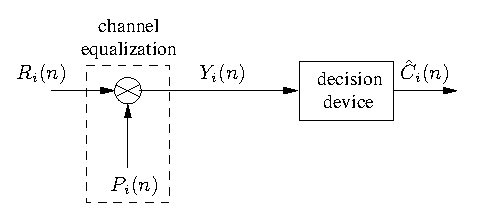
\includegraphics[width=0.6\linewidth]{equalization.eps}
\caption{Block diagram of an OFDM receiver\label{fig:equalization}}
\end{figure}
%
Intuitively, the simplest method for the design of the equalizer coefficients, is to perform a pure channel inversion, know as \gls{zf} criterion. The equalizer coefficients are then given by
%
\begin{equation}
\label{eqn:EqCoeff}
 P_i(n)=\frac{1}{H_i(n)},
\end{equation}
%
while the DFT output takes the form
%
\begin{equation}
\label{eqn:DFToutEq}
 Y_i(n)=\frac{R_i(n)}{H_i(n)}=C_i(n) + \frac{W_i(n)}{H_i(n)},\ 0\leq n \leq N-1.
\end{equation}
%
From (\ref{eqn:DFToutEq}) it can be noticed that ZF equalization is capable of totally compensating for any distortion induced by the wireless channel. However, the noise power at the equalizer output is given by $\sigma_w^2/|H_i(n)|^2$ and may be excessively large over deeply faded subcarriers characterized by low channel gains. 

Inherent system requirement for ZF equalizer is the knowledge of the channel transfer function $H_i(n)$. Therefore, in many wireless \gls{ofdm} systems, sequence of data symbols is preceded by several reference OFDM symbols (preambles) known to the receiver, forming the \textbf{OFDM frame}. Typical frame structure is shown in {~\cref{fig:frame}} where preambles are typically used for \textbf{synchronization} and/or \textbf{channel estimation} purposes.
%
\begin{figure}[thb]
\centering
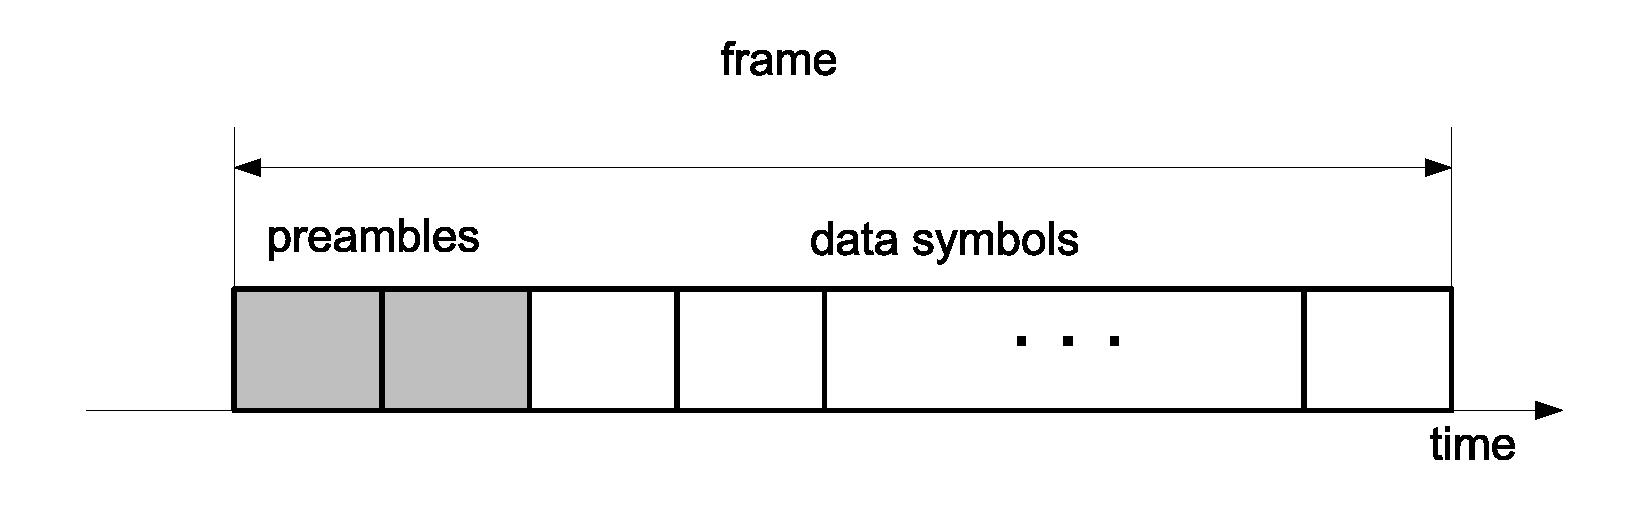
\includegraphics[width=0.6\linewidth]{framefinal}
\caption{Frame structure\label{fig:frame}}
\end{figure}
%
In typical fixed wireless standards as WLAN, it can be assumed that the channel remains static over frame duration, i.e., $H_i(n) = H(n)$ for $i = 1,\ldots,I$, where $I$ is the total number of OFDM symbols within one frame. Then, channel estimates obtained from the preambles can be used to coherently detect the entire payload.

Assuming that the OFDM frame has one preamble with index $i=p=1$, the output of the DFT block (\ref{eqn:DFTout}) can be written as
%
\begin{equation}
\label{eqn:DFToutPream}
 R_p(n)=H(n)C_p(n) + W_p(n),\ 0\leq n \leq N-1
\end{equation}
%
where $C_p(n)$ are complex data symbols \textbf{known} to the receiver. Then, estimates of the {channel frequency response}\index{Channel frequency response} $\hat{H}(n)$ can be obtained as
%
\begin{equation}
\label{eqn:Estimates}
 \hat{H}(n) = \frac{R_p(n)}{C_p(n)}=H(n) + \frac{W_p(n)}{C_p(n)},\ 0\leq n \leq N-1.
\end{equation}
%
On the other hand, in applications characterized by relatively high mobility as those envisioned by the \gls{lte} standard, the channel response undergoes significant variations over one frame and must continuously be tracked to maintain reliable data detection. In this case, in addition to initial reference blocks, known symbols called pilots are normally inserted into the payload section of the frame at some convenient positions. These pilots are scattered in both time and frequency directions (i.e., they are positioned over different blocks and different subcarriers), and are used as reference values for channel estimation and tracking.

In order to assess and compare the influence of system impairments on different data rates supported in \gls{ofdm} systems, a short survey of commonly used coherent modulation techniques and their performance evaluation in \gls{awgn} channel are given in the next section.

\section{Digital Modulations Used in OFDM Systems}\label{sec:cohmod}
%
Consider some digital information that is given by a finite bit sequence. To transmit this information over a physical, analog channel by a passband signal (on the \gls{rf} frequency) we need a mapping rule between the set of bit sequences and the set of possible signals or constellation points on the complex plane, as shown in ~\cref{fig:PSKconstell}. Such a mapping rule is called a digital modulation scheme. An example is shown in~\cref{fig:bpsk-passband}, where the red signal represent a logical $1$ and the blue signal a logical $0$. The signal frequency is the carrier frequency, i.e., it is the passband signal. In \acrlong{bb}, this would be represented by one complex symbol per passband signal. To go from the passband to the \gls{bb}, the carrier frequency is removed from the passband signal, thus the only thing remaining is the amplitude and phase contributions, i.e., the complex symbol. 

\begin{figure}
    
    \begin{subfigure}[t]{0.6\textwidth}
    \centering
    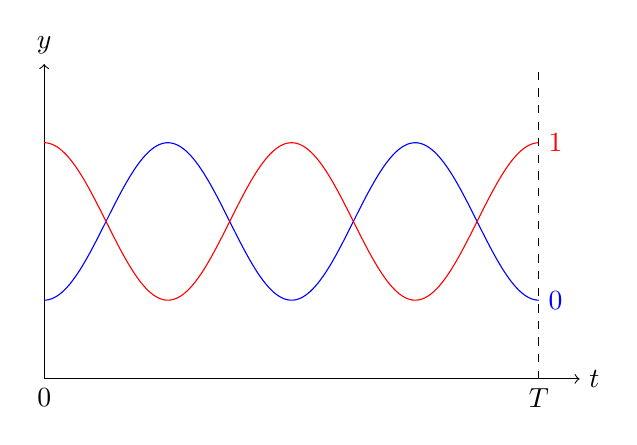
\begin{tikzpicture}
  % Parameters
  \def\phaseA{180} % Phase in degrees for cosine A
  \def\phaseB{0} % Phase in degrees for cosine B
  \def\frequencyA{2} % Frequency in Hz for cosine A
  \def\frequencyB{2} % Frequency in Hz for cosine B
  \def\amplitudeA{1} % Amplitude for cosine A
  \def\amplitudeB{1} % Amplitude for cosine B
  
  % Plot cosine function A
  \draw[->] (0,-2) -- (6.8,-2) node[right] {$t$};
  \draw[->] (0,-2) -- (0,2) node[above] {$y$};
  \draw[domain=0:2*pi,samples=200,smooth,variable=\t,blue] plot ({\t},{\amplitudeA*cos(\frequencyA*\t r + \phaseA)});
  
  % Plot cosine function B
  \draw[domain=0:2*pi,samples=200,smooth,variable=\t,red] plot ({\t},{\amplitudeB*cos(\frequencyB*\t r + \phaseB)});


  \node[right, red] at (2*pi,1) {$1$};
  \node[right, blue] at (2*pi,-1) {$0$};

  \node[below] at (2*pi,-2) {$T$};
  
   \node[below] at (0,-2) {$0$};
  % Vertical dashed line at t = 2*pi
  \draw[dashed] (2*pi,-2) -- (2*pi,2);
  
\end{tikzpicture}
    \caption{BSPK passband signal representation.}
    \label{fig:bpsk-passband}
\end{subfigure}
\hfill
        \begin{subfigure}[t]{0.3\textwidth}
        \centering
    % BPSK constellation
\begin{tikzpicture}[x=1.3cm,y=1.3cm]
    % Draw axes
    \draw[->] (-1.5,0) -- (1.5,0) node[right] {$I$};
    \draw[->] (0,-1.5) -- (0,1.5) node[above] {$Q$};
    
    % Draw constellation points
    \draw[fill=red] (1,0) circle (0.08) node[above right] {\footnotesize 1};
    \draw[fill=blue] (-1,0) circle (0.08) node[above left] {\footnotesize 0};

    % DRAW UNIT CIRCLE
    \draw[dashed] (0,0) circle (1);
    
    % Draw labels
    %\node[above] at (0,1.7) {BPSK};
    %\node[below] at (0,-1.7) {Gray-coded bits: 0, 1};
\end{tikzpicture}
\caption{BSPK complex \gls{bb} signal representation.}
    \label{fig:bpsk-passband}
\end{subfigure}
\end{figure}

A linear digital modulation scheme is characterized by the complex baseband signal~\cite{RFSDR}
%
\begin{equation}
\label{eqn:timetime}
C(t) = \sum_iC_ig(t-kT),
\end{equation}
%
where $C_i$ is a given constellation point (complex) and $g(t)$ is a pulse shape used for transmission. In~\cref{fig:bpsk-passband}, the pulse shape is a rectangular window in the time domain, meaning that the signal is transmitted over a finite time, the symbol time $T$. 
Since mapping is usually performed in digital domain, we will keep discrete domain representation of modulated complex symbols for further simplification. In the following, we will resume some of the coherent modulation schemes typically used in \gls{ofdm} systems.






\subsection{Phase Shift Keying (PSK)}
\gls{psk} or Multiple \gls{psk} (M-\gls{psk}) modulation, where $M$ is the number of constellation points, is characterized that all signal information is put into the phase of the transmitted signal, preserving constant envelope property (the amplitude between symbols are constant). The M-\gls{psk} complex symbol $C_i$ can be written as
%
\begin{equation}
\label{eqn:PSKmod}
C_i=\sqrt{S}e^{j(\frac{2\pi m}{M} + \theta_0)},\ m = 0,1,\ldots,M-1,
\end{equation}
%
where $S$ is the average signal power and $\theta_0$ is an arbitrary constant phase. Constellation diagrams for $M=2,4,8$, i.e., \gls{bpsk}, \gls{qpsk} or 4-\gls{psk} and 8-\gls{psk}, respectively, when $\theta_0=0$, are shown in~\cref{fig:PSKconstell}.

\begin{figure}[thb]
\centering
    \begin{subfigure}[t]{0.3\textwidth}
    % BPSK constellation
\begin{tikzpicture}[x=1.3cm,y=1.3cm]
    % Draw axes
    \draw[->] (-1.5,0) -- (1.5,0) node[right] {$I$};
    \draw[->] (0,-1.5) -- (0,1.5) node[above] {$Q$};
    
    % Draw constellation points
    \draw[fill=black] (1,0) circle (0.05) node[above right] {\footnotesize 1};
    \draw[fill=black] (-1,0) circle (0.05) node[above left] {\footnotesize 0};

    % DRAW UNIT CIRCLE
    \draw[dashed] (0,0) circle (1);
    
    % Draw labels
    %\node[above] at (0,1.7) {BPSK};
    %\node[below] at (0,-1.7) {Gray-coded bits: 0, 1};
\end{tikzpicture}
    \caption{BPSK constellation diagram}\label{fig:BPSK}
    \end{subfigure}
\hfill
    \begin{subfigure}[t]{0.3\textwidth}
    % QPSK constellation
\begin{tikzpicture}[x=1.3cm,y=1.3cm]
% Draw axes
    \draw[->] (-1.5,0) -- (1.5,0) node[right] {$I$};
    \draw[->] (0,-1.5) -- (0,1.5) node[above] {$Q$};
    
  \foreach \i/\j/\k in {0.707/-0.707/01, -0.707/-0.707/00} {
    \node[circle,fill,inner sep=1.5pt,label={[font=\footnotesize]below:$\k$}] at (\i,\j) {};
  }
  \foreach \i/\j/\k in {0.707/0.707/11, -0.707/0.707/10} {
    \node[circle,fill,inner sep=1.5pt,label={[font=\footnotesize]above:$\k$}] at (\i,\j) {};
  }
  %\node[align=center] at (0,-2) {QPSK Constellation};
  % DRAW UNIT CIRCLE
    \draw[dashed] (0,0) circle (1);
    
    % Draw labels
    %\node[above] at (0,1.9) {QPSK};
    %\node[below] at (0,-1.7) {Gray-coded bits: 00, 01, 11, 10};
    
\end{tikzpicture}
    \caption{QPSK(4-PSK) constellation diagram}\label{fig:QPSK}
    \end{subfigure}
\hfill
    \begin{subfigure}[t]{0.3\textwidth}
    % 16-QAM constellation
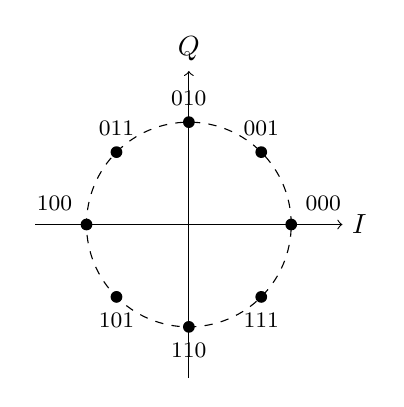
\begin{tikzpicture}[x=1.3cm,y=1.3cm]
 % Draw axes
    \draw[->] (-1.5,0) -- (1.5,0) node[right] {$I$};
    \draw[->] (0,-1.5) -- (0,1.5) node[above] {$Q$};

     % DRAW UNIT CIRCLE
    \draw[dashed] (0,0) circle (1);
    
  \foreach \angle/\bits in {225/101, 270/110, 315/111} {
    \draw (\angle:1) node[circle,fill,inner sep=1.5pt,label={[font=\footnotesize]below:$\bits$}] {};
  }

  \foreach \angle/\bits in {45/001, 90/010, 135/011} {
    \draw (\angle:1) node[circle,fill,inner sep=1.5pt,label={[font=\footnotesize]above:$\bits$}] {};
  }

  \draw (0:1) node[circle,fill,inner sep=1.5pt,label={[font=\footnotesize]above right:$000$}] {};

  \draw (180:1) node[circle,fill,inner sep=1.5pt,label={[font=\footnotesize]above left:$100$}] {};

  % \foreach \angle/\bits in {0/000, 45/001, 90/010, 135/011, 180/100, 225/101, 270/110, 315/111} {
  %   \draw (\angle:1) node[circle,fill,inner sep=1.5pt,label={[font=\footnotesize]below:$\bits$}] {};
  % }

  %\node[align=center] at (0,-2) {8-PSK Constellation};
\end{tikzpicture}
    \caption{8-PSK constellation diagram}
    \label{fig:8PSK}
    \end{subfigure}
\caption{Gray-coded constellation diagrams}
\label{fig:PSKconstell}
\end{figure}

%
% \begin{figure}[thb]
% \centering
%     \begin{subfigure}[t]{0.3\textwidth}
%     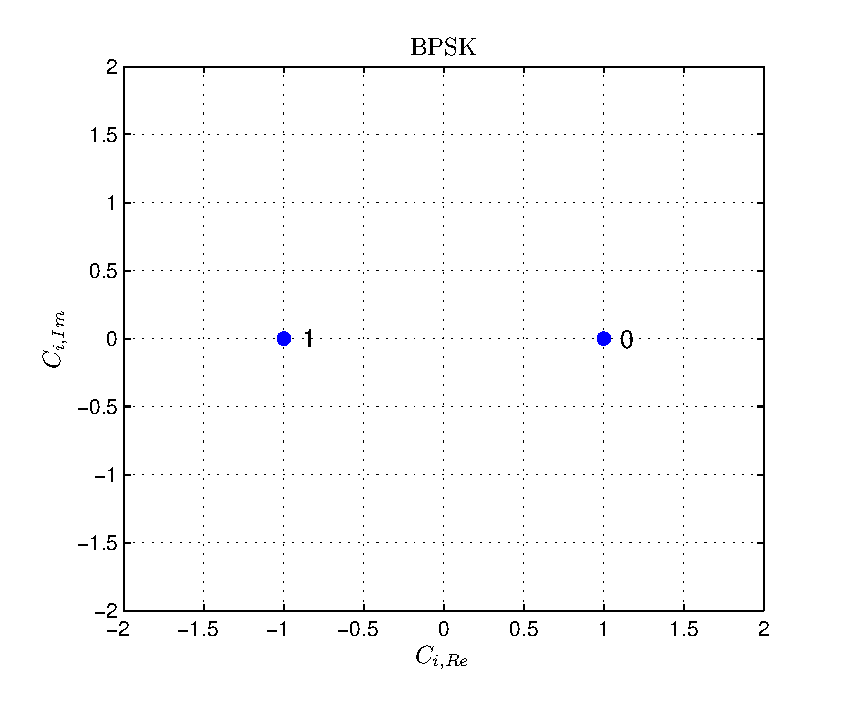
\includegraphics[width=\linewidth]{bpskmapp}
%     \caption{BPSK constellation diagram}\label{fig:BPSK}
%     \end{subfigure}
% \hfill
%     \begin{subfigure}[t]{0.3\textwidth}
%     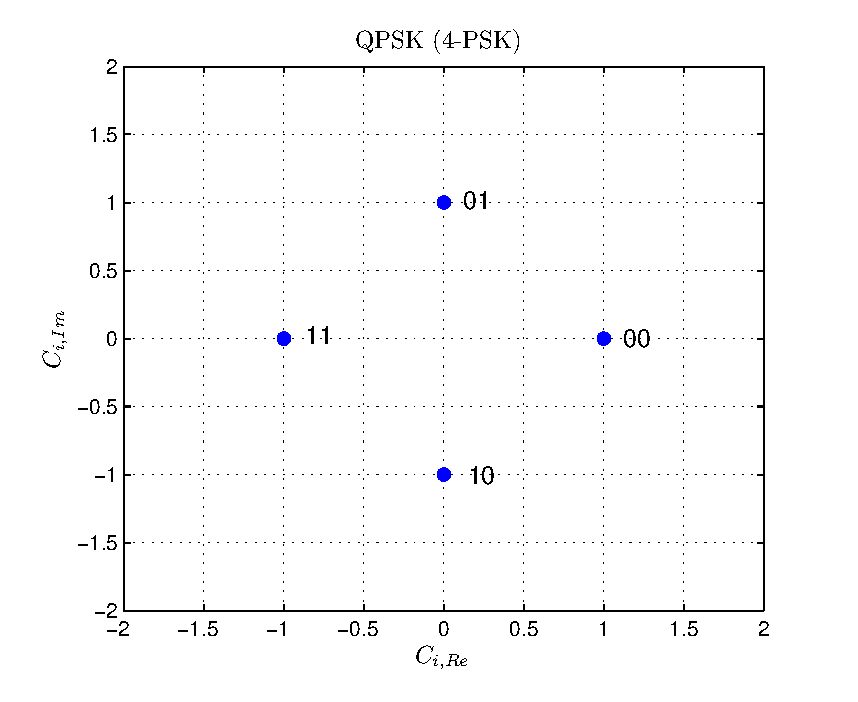
\includegraphics[width=\linewidth]{qpskmapp}
%     \caption{QPSK(4-PSK) constellation diagram}\label{fig:QPSK}
%     \end{subfigure}
% \hfill
%     \begin{subfigure}[t]{0.3\textwidth}
%     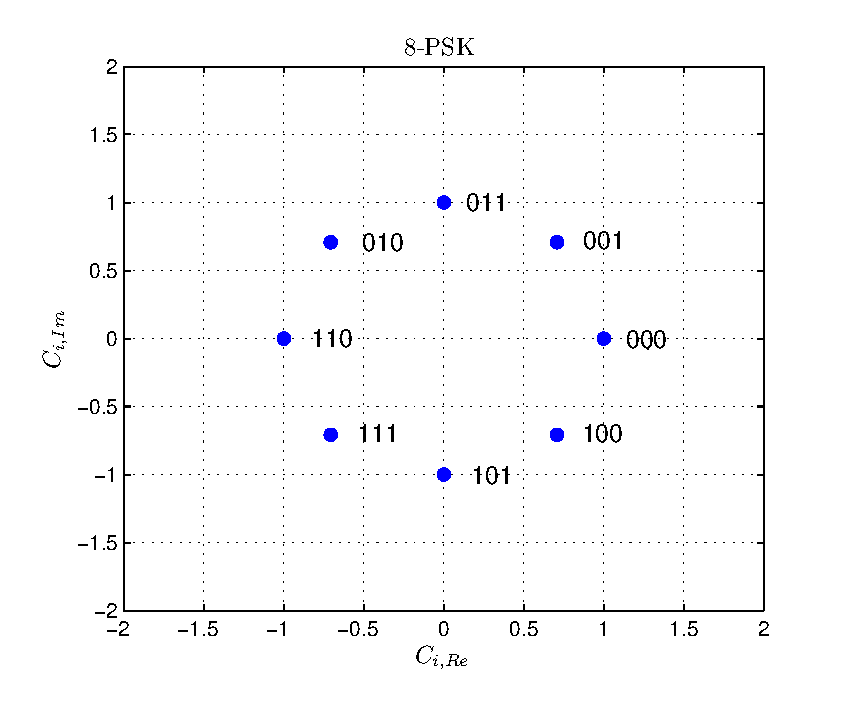
\includegraphics[width=\linewidth]{8pskmapp}
%     \caption{8-PSK constellation diagram}
%     \label{fig:8PSK}
%     \end{subfigure}
% \caption{Gray-coded M-PSK constellation diagrams}
% \label{fig:PSKconstell}
% \end{figure}
%
The simplest \gls{psk} modulation format is \gls{bpsk}, where a logical \glqq 1\grqq\ is encoded as $0$ phase, and a logical \glqq 0\grqq\ is coded as a phase of $\pi$. Then, the modulated symbol, defined in (\ref{eqn:PSKmod}), can be written as
%
\begin{equation}
\label{eqn:BPSKmod}
C_i=\pm \sqrt{S}
\end{equation}
%
with constellation diagram shown in ~\cref{fig:BPSK}. M-\gls{psk} constellation diagram for 4-\gls{psk} ($2$ bits mapped into $4=2^2$ phases) and 8-\gls{psk} ($3$ bits mapped into $8=2^3$ phases), are shown in ~\cref{fig:QPSK} and ~\cref{fig:8PSK}, respectively. Note that they are optimized to minimize the \gls{ber}, resulting in the gray-coded M-PSK constellation, i.e., adjacent constellation points differ in one bit as in ~\cref{fig:PSKconstell}. The BER is defined as the ratio between the number of successfully received to the number of total transmitted information bits and is usually taken as a measure of modulation quality. 

% For \gls{bpsk} in \gls{awgn} it is given as \cite{WiComGoldsmith}
% %
% \begin{equation}
% \label{eqn:BPSKmodBER}
% p_{b,BPSK} = Q\left(\sqrt{\frac{2E_b}{N_0}}\right), 
% \end{equation}
% %
% where $\frac{E_b}{N_0}$ is the SNR\index{SNR} per bit and $Q(x)$ is defined as
% %
% \begin{equation}
% \label{eqn:Qfunction}
% Q(x)=\frac{1}{2}\operatorname{erfc}\left(\frac{x}{\sqrt{2}}\right),
% \end{equation}
% %
% where
% %
% \begin{equation}
% \label{eqn:Erfcfunction}
% \operatorname{erfc}(x)=\frac{2}{\sqrt{\pi}}\int_x^{\infty}{e^{-y^2}dy}
% \end{equation}
% %
% is the complementary error function ($\operatorname{erfc}$).
% For higher order M-\gls{psk}, where $M>4$, the symbol error rate (SER)\index{SER} can be expressed as
% %
% \begin{equation}
% \label{eqn:PSKmodBER}
% p_{s,M-PSK} = 2Q\left( \sqrt{\frac{2E_b\log_2M}{N_0}}\sin{\frac{\pi}{M}}\right),
% \end{equation}
% %
% where 
% \begin{equation*}
% \frac{E_s}{N_0}=\frac{E_b\log_2M}{N_0}
% \end{equation*}
% is the \gls{snr} per symbol. For Gray-coded modulations the \gls{ber} in the high \gls{snr} regime for each modulation is approximately
% \begin{equation*} 
% p_{b,M-PSK} \approx \frac{p_{s,M-PSK}}{\log_2M}.
% \end{equation*}

\subsection{QuaIdrature Amplitude Modulation (QAM)}
\gls{qam} is a bandwidth efficient signaling scheme that, unlike M-\gls{psk} does not possess a
constant envelope property, thus offering higher bandwidth efficiency, i.e., more bits per second (bps) can be transmitted in a given frequency bandwidth. 






\begin{figure}[hbtp]
    \centering
    \begin{subfigure}[t]{0.3\textwidth}\centering
    \begin{tikzpicture}[x=1.6cm,y=1.6cm]
    % Define the constellation points
    \foreach \i in {0,...,1} {
        \foreach \j in {0,...,1} {
            \pgfmathsetmacro{\x}{-0.5 + \i}
            \pgfmathsetmacro{\y}{-0.5 + \j}
            \node[draw, circle, fill=black, inner sep=0.5pt] at (\x, \y) {};
        }
    }
    % Add axes
    \draw[->] (-1.125,0) -- (1.125,0) node[right] {$I$};
    \draw[->] (0,-1.125) -- (0,1.125) node[above] {$Q$};
    \end{tikzpicture}
    \caption{4-QAM}
    \label{fig:4QAM}
    \end{subfigure}\hfill
    \begin{subfigure}[t]{0.3\textwidth}\centering
        \begin{tikzpicture}[x=0.8cm,y=0.8cm]
    % Define the constellation points
    \foreach \i in {0,...,3} {
        \foreach \j in {0,...,3} {
            \pgfmathsetmacro{\x}{-1.5 + \i}
            \pgfmathsetmacro{\y}{-1.5 + \j}
            \node[draw, circle, fill=black, inner sep=0.5pt] at (\x, \y) {};
        }
    }
    % Add axes
    \draw[->] (-2.25,0) -- (2.25,0) node[right] {$I$};
    \draw[->] (0,-2.25) -- (0,2.25) node[above] {$Q$};
    \end{tikzpicture}
    \caption{16-QAM}
    \label{fig:16QAM}
    \end{subfigure}\hfill
    \begin{subfigure}[t]{0.3\textwidth}\centering
    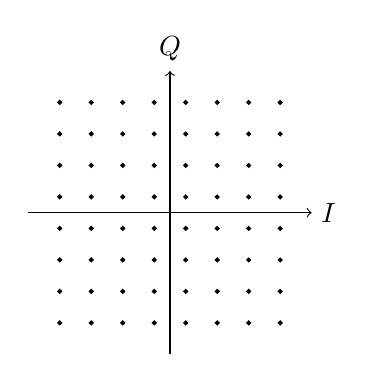
\begin{tikzpicture}[x=0.4cm,y=0.4cm]
    % Define the constellation points
    \foreach \i in {0,...,7} {
        \foreach \j in {0,...,7} {
            \pgfmathsetmacro{\x}{-3.5 + \i}
            \pgfmathsetmacro{\y}{-3.5 + \j}
            \node[draw, circle, fill=black, inner sep=0.5pt] at (\x, \y) {};
        }
    }
    % Add axes
    \draw[->] (-4.5,0) -- (4.5,0) node[right] {$I$};
    \draw[->] (0,-4.5) -- (0,4.5) node[above] {$Q$};
    \end{tikzpicture}
    \caption{64-QAM}
    \label{fig:64QAM}
    \end{subfigure}
    
    \begin{subfigure}[t]{0.3\textwidth}\centering
    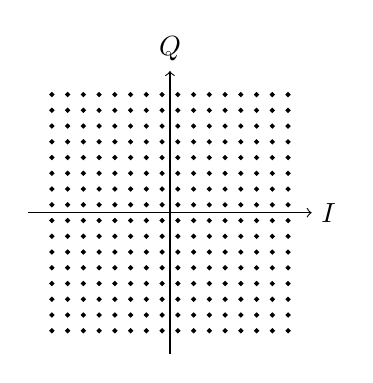
\begin{tikzpicture}[x=0.2cm,y=0.2cm]
        % Define the constellation points
        \foreach \i in {0,...,15} {
            \foreach \j in {0,...,15} {
                \pgfmathsetmacro{\x}{-7.5 + \i}
                \pgfmathsetmacro{\y}{-7.5 + \j}
                \node[draw, circle, fill=black, inner sep=0.5pt] at (\x, \y) {};
            }
        }
        % Add axes
        \draw[->] (-9,0) -- (9,0) node[right] {$I$};
        \draw[->] (0,-9) -- (0,9) node[above] {$Q$};
        \end{tikzpicture}
        \caption{256-QAM}
    \label{fig:256QAM}
    \end{subfigure}\hfill
     \begin{subfigure}[t]{0.3\textwidth}\centering
    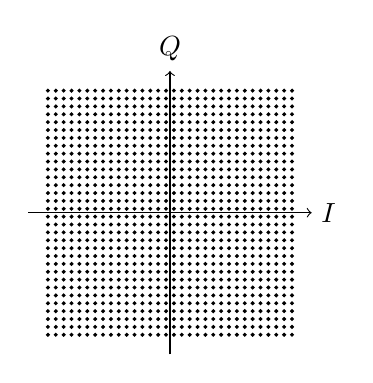
\begin{tikzpicture}[x=0.1cm,y=0.1cm]
        % Define the constellation points
        \foreach \i in {0,...,31} {
            \foreach \j in {0,...,31} {
                \pgfmathsetmacro{\x}{-15.5 + \i}
                \pgfmathsetmacro{\y}{-15.5 + \j}
                \node[draw, circle, fill=black, inner sep=0.1pt] at (\x, \y) {};
            }
        }
        % Add axes
        \draw[->] (-18,0) -- (18,0) node[right] {$I$};
        \draw[->] (0,-18) -- (0,18) node[above] {$Q$};
        \end{tikzpicture}
        \caption{1024-QAM}
    \label{fig:1024QAM}
    \end{subfigure}\hfill
     \begin{subfigure}[t]{0.3\textwidth}\centering
    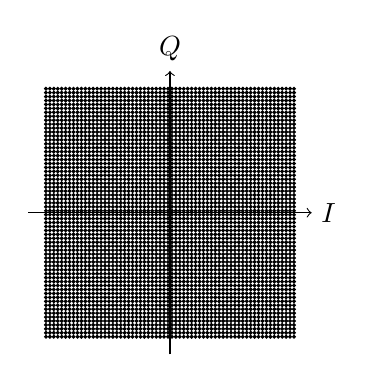
\begin{tikzpicture}[x=0.05cm,y=0.05cm]
        % Define the constellation points
        \foreach \i in {0,...,63} {
            \foreach \j in {0,...,63} {
                \pgfmathsetmacro{\x}{-31.5 + \i}
                \pgfmathsetmacro{\y}{-31.5 + \j}
                \node[draw, circle, fill=black, inner sep=0pt] at (\x, \y) {};
            }
        }
        % Add axes
        \draw[->] (-36,0) -- (36,0) node[right] {$I$};
        \draw[->] (0,-36) -- (0,36) node[above] {$Q$};
        \end{tikzpicture}
        \caption{4096-QAM}
    \label{fig:4096QAM}
    \end{subfigure}
    \caption{QAM constellation diagrams}
\label{fig:QAMconstell}
\end{figure}

\Gls{qam} modulated signals for $M$ constellation points can be written as
%
\begin{equation*}
C_i=\sqrt{S}K(X_i + jY_i),
\end{equation*}
%
where $X_i, Y_i \in \left\lbrace\pm 1, \pm 3,\ldots,\sqrt{M}-1 \right\rbrace$ and $K$ is a scaling factor for normalizing the average power for all constellations to $S$. The $K$ value for various constellations is shown in Table~\ref{tab:param}. Corresponding \gls{qam} constellation diagrams for 4-\gls{qam} ($2$ bits mapped into $4=2^2$ points), 16-\gls{qam} ($4$ bits mapped into $16=2^4$ points), 64-\gls{qam} ($6$ bits mapped into $64=2^6$ points), and 256-\gls{qam} ($8$ bits mapped into $16=2^8$ points), are shown in ~\cref{fig:QAMconstell}. It can be noticed that 4-\gls{qam} corresponds to \gls{qpsk} with constant phase shift $\theta_0 =\pi/4$. 

\Gls{qam} schemes are used in several typical wireless digital communications specifications for a long time. A trend is the drastic increase in modulation depth as can be seen in \cref{tab:wifi-qam}.


% \begin{figure}[thb]
% \centering

% \begin{subfigure}[b]{0.42\textwidth}
%     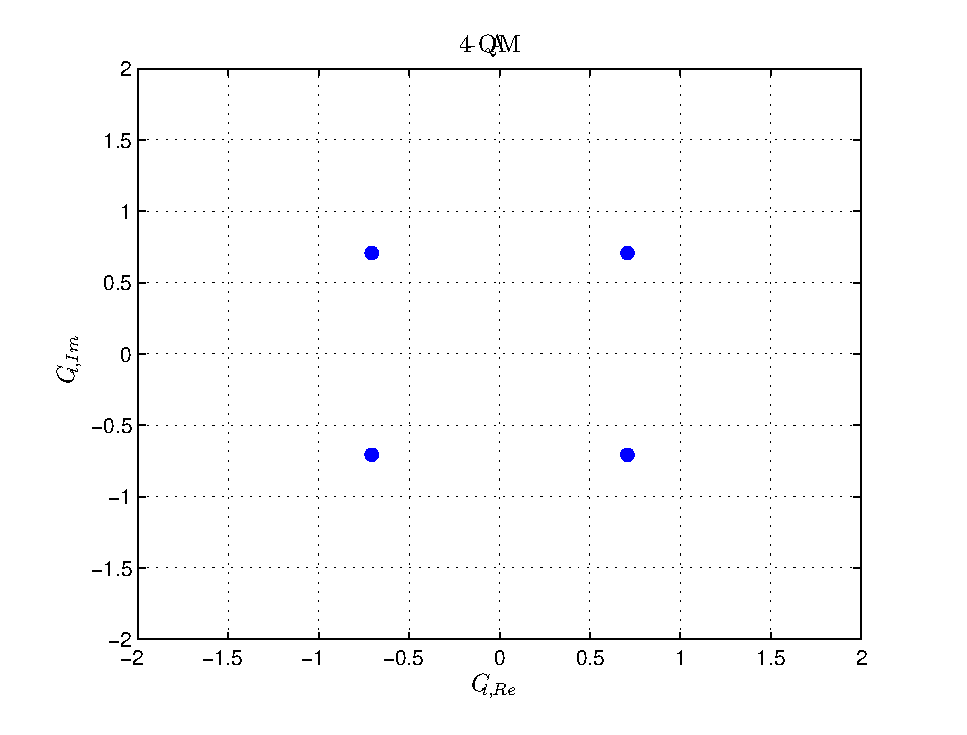
\includegraphics[width=\linewidth]{figs/4-QAM.eps}
%     \caption{4-QAM constellation diagram}
%     \label{fig:4QAM}
%     \end{subfigure}%
% \begin{subfigure}[b]{0.42\textwidth}
%     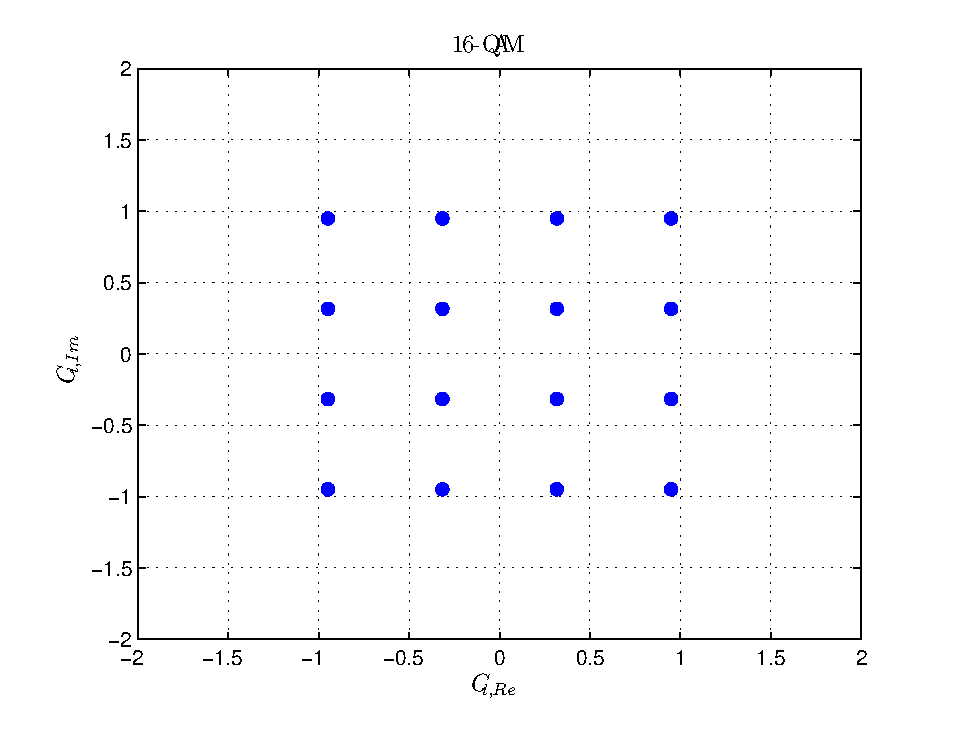
\includegraphics[width=\linewidth]{figs/16-QAM.eps}
%     \caption{16-QAM constellation diagram}
%     \label{fig:16QAM}
%     \end{subfigure}

% \begin{subfigure}[b]{0.42\textwidth}
%     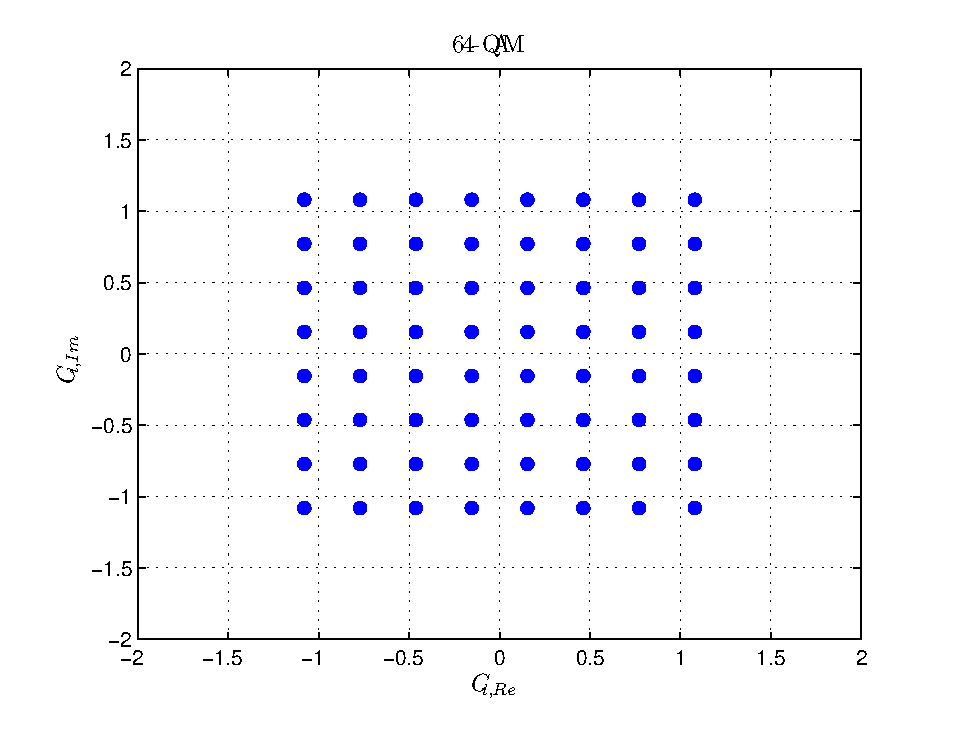
\includegraphics[width=\linewidth]{figs/64-QAM.eps}
%     \caption{64-QAM constellation diagram}
%     \label{fig:64QAM}
%     \end{subfigure}%
% \begin{subfigure}[b]{0.42\textwidth}
%     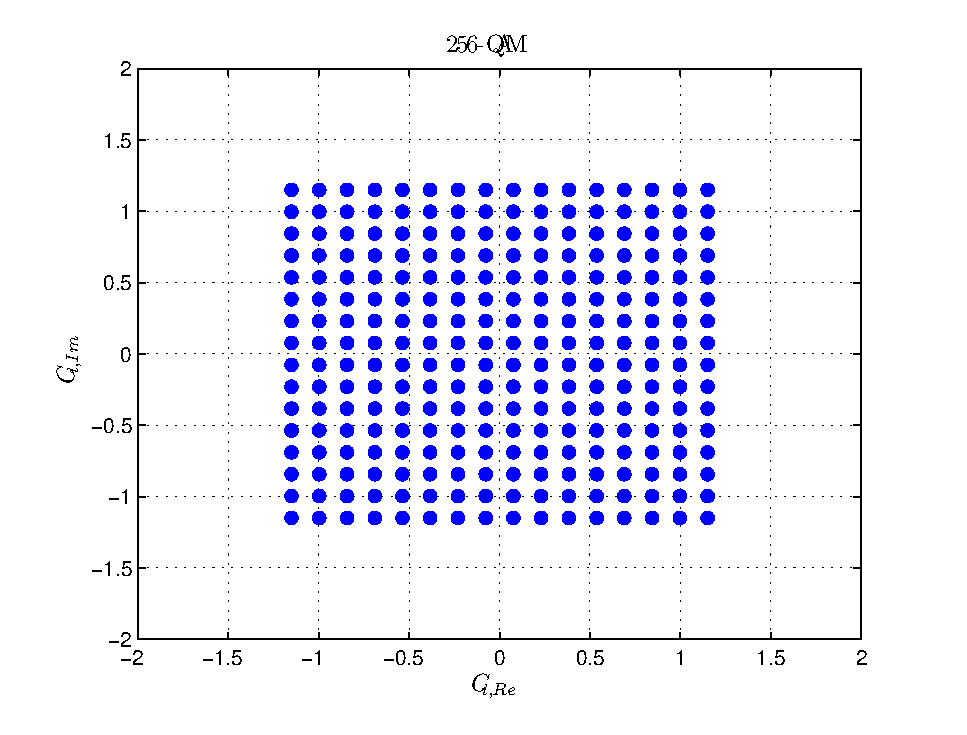
\includegraphics[width=\linewidth]{figs/256-QAM.eps}
%     \caption{256-QAM constellation diagram}
%     \label{fig:256QAM}
%     \end{subfigure}
% %%\end{center}
% \caption{QAM constellation diagrams}
% \label{fig:QAMconstell}
% \end{figure}
%

%
\begin{table}[htb]
\centering
\scriptsize
\renewcommand\arraystretch{1.6}
\caption{Modulation dependent parameters}\label{tab:param}
\begin{tabular}{ p{3cm} p{3cm} p{3cm}}\toprule
Modulation&Number of bits $m$&$K$\\\midrule
4-QAM&2&$1/\sqrt{2}$\\
16-QAM&4&$1/\sqrt{10}$\\
64-QAM&6&$1/\sqrt{42}$\\
256-QAM&8&$1/\sqrt{170}$\\\bottomrule
\end{tabular}
\end{table}
%
% The \gls{ser} for \gls{qam} modulations can be expressed as
% %
% \begin{equation*}
% %\label{eqn:MQAMmodSER}
% p_{s,M-QAM} = 1-\left( 1-2\left( 1-\frac{1}{\sqrt{M}}\right)Q\left( \sqrt{3\frac{E_b\log_2 M}{(M-1)N_0}}\right) \right) ^2.
% \end{equation*}
% %
% where $Q(x)$ is defined in (\ref{eqn:Qfunction}). For Gray-coded modulations  the \gls{ber} in the high \gls{snr} regime for each modulation is, as for M-PSK case, approximately
% \begin{equation}
% \label{eqn:MQAMmodBER}
% p_{b,M-QAM} \approx \frac{p_{s,M-QAM}}{\log_2M}.
% \end{equation}


\begin{table}[hbtp]
    \centering
    \scriptsize
    \caption{Overview of maximum modulation depth in Wi-Fi.~\cite{enwiki:1210657347}}
    \label{tab:wifi-qam}
\renewcommand\arraystretch{1.6}
    \begin{tabular}{l l l r}
    \toprule
    Wi-Fi standard & IEEE standard & Modulation Depth & bits per symbol\\
    \midrule
    Wi-Fi 5 & 802.11ac   &  256-QAM& 8\\
    Wi-Fi 6(E) & 802.11ax   &  1024-QAM & 10\\
    Wi-Fi 7 & 802.11be   &  4096-QAM &12\\
    Wi-Fi 8 & 802.11bn   &  8192-QAM &13\\
    \bottomrule
    \end{tabular}
    
\end{table}

